\documentclass[]{mwart}

\usepackage{polski}
\usepackage[utf8]{inputenc}

\usepackage{amsthm}
\usepackage{amsmath}
\usepackage{amssymb}

\usepackage{mdframed}
\usepackage{hyperref}
\usepackage[draft%      % dla obrazkow zakomentowac draft
]{graphicx}  
\usepackage{url}
\usepackage{enumitem}
\usepackage{verbatim}



\usepackage{caption}    
\usepackage{float}      



\usepackage{fancyhdr}
\pagestyle{fancy}
\fancyhf{}

\fancyhead[L]{
\includegraphics[height=0.666cm]{wspolne_dla_wszystkich/logo_projektu.png}}
\fancyhead[C]{\textit{Poprawa jakości zdjęć}}
\fancyhead[R]{
\includegraphics[height=0.9cm]{wspolne_dla_wszystkich/logo_uczelni.png}}
\fancyfoot[C]{\thepage}

\setlength{\headheight}{20pt}  



\usepackage{listings}
\usepackage{xcolor} 




\begin{document}
\thispagestyle{empty}

\begin{figure}[h]
    \centering
    
\includegraphics[width=1\textwidth]{wspolne_dla_wszystkich/logo_uczelni.png}
\end{figure}


\begin{center}
    {\LARGE \textbf{Poprawa jakości skanów zdjęć wykonanych techniką analogową
        }} \\[0.3cm]
    {\large \textbf{Raport II}} \\[0.2cm]
    \textit{projekt realizowany pod opieką prof. dr hab. inż. Artura Przelaskowskiego}

\end{center}

\begin{figure}[h]
    \centering
    
\includegraphics[width=1\textwidth]{wspolne_dla_wszystkich/logo_projektu.png}
\end{figure}

\vfill
\begin{abstract}
    Raport 2 projektu poprawy jakości cyfrowych skanów zdjęć wykonanych techniką analogową przez grupę nr 9 (wtorkową z godziny 18)
    w składzie:  Bartosz Wójcik, Katarzyna Szwed, Natalia Szymańska,
    Patrycja Szałajko, Aleksandra Wójcik, Karol Sęk, Michał Juszkiewicz, Filip Sajko.

    W tym raporcie zredefiniujemy cel naszego projektu i opiszemy problem z którym się mierzymy.
    Przedstawimy ponadto wstępną wersję naszego programu i zademonstrujemy jego skuteczność.
\end{abstract}

\newpage
\tableofcontents{}

\newpage

\section{Cel projektu}
W związku ze słusznymi uwagami i wskazówkami, podjęliśmy decyzję o ukonkretyzowaniu celu naszego projektu.
Skupimy się przede wszystkim na poprawianiu defektów cyfrowych skanów zdjęć analogowych.
Staramy się trafić do dwóch (niekoniecznie rozłącznych) grup osób --
współczesnych fanów fotografii analogowej (będącą dla amatora niełatwą sztuką) i posiadaczy pękatych
archiwów zdjęć rodzinnych chcących je zachować i cyfrowo utrwalić.

\section{Zdjęcia, zdjęcia!}
Profilowym zdjęciem dla nas jest portret -- tak indywidualny jak i grupowy.
Jest to typ zdjęć najbardziej popularny w rodzinnych albumach -- mnogość w nich zdjęć z ważnych
dla danej familli wydarzeń: chrztów, wesel czy pogrzebów... Służą one utrwaleniu wspomnień oraz pamięci
po krewnych i bliskich, którzy już odeszli... A więc noszących dużą wartość emocjonalną dla ich posiadacza.

Przykładem takiej osoby jest nasza koleżanka Ola -- wraz z jej rodzinnym albumem.

\section{Problemy}
Wykonywanie, a następnie `ucyfrowienie' zdjęcia w technice analogowej wiąże się z różnymi trudnościami,
które mogą znacząco obniżyć jakość zdjęcia -- a z tym satysfakcje jego posiadacza. Głównymi problemami,
którym będziemy przeciwdziałać, będą niedoświetlenie zdjęcia i zanieczyszczenia powietrza osadzające
się na oryginalnym zdjęciu i skanerze podczas procesu zmiany informacji z analogowej na cyfrową.

\subsection{Niedoświetlenie} % tak wiem bartek bedziesz krzyczał. ale poezja to poezja, e viva latre
Niedoświetlenie jest problemem trudnym -- zwłaszcza dla fanów-amatorów techniki analogowej.
Zasadnicza większość klasycznych aparatów nie posiada zaawansowanej mechaniki automatycznie wybierającej
odpowiednie ustawienia aparatu, a brak możliwości podglądu tego, jak dane zdjęcie wyszło, często doprowadza
do sytuacji, gdzie po wielu dniach okazuje się, że na zdjęciu chwili, którą fotograf chciał uchwycić i utrwalić,
niewiele widać, bo przez złe ustawienia większość szczegółów jest niewidoczna...\footnote{Jest to problem, który szeroko
    wraz z przykładami i analizą numeryczną opisywaliśmy w raporcie pierwszym.}

Dla przykładu przypomnijmy:
\newpage
\begin{figure}[H]
    \centering
    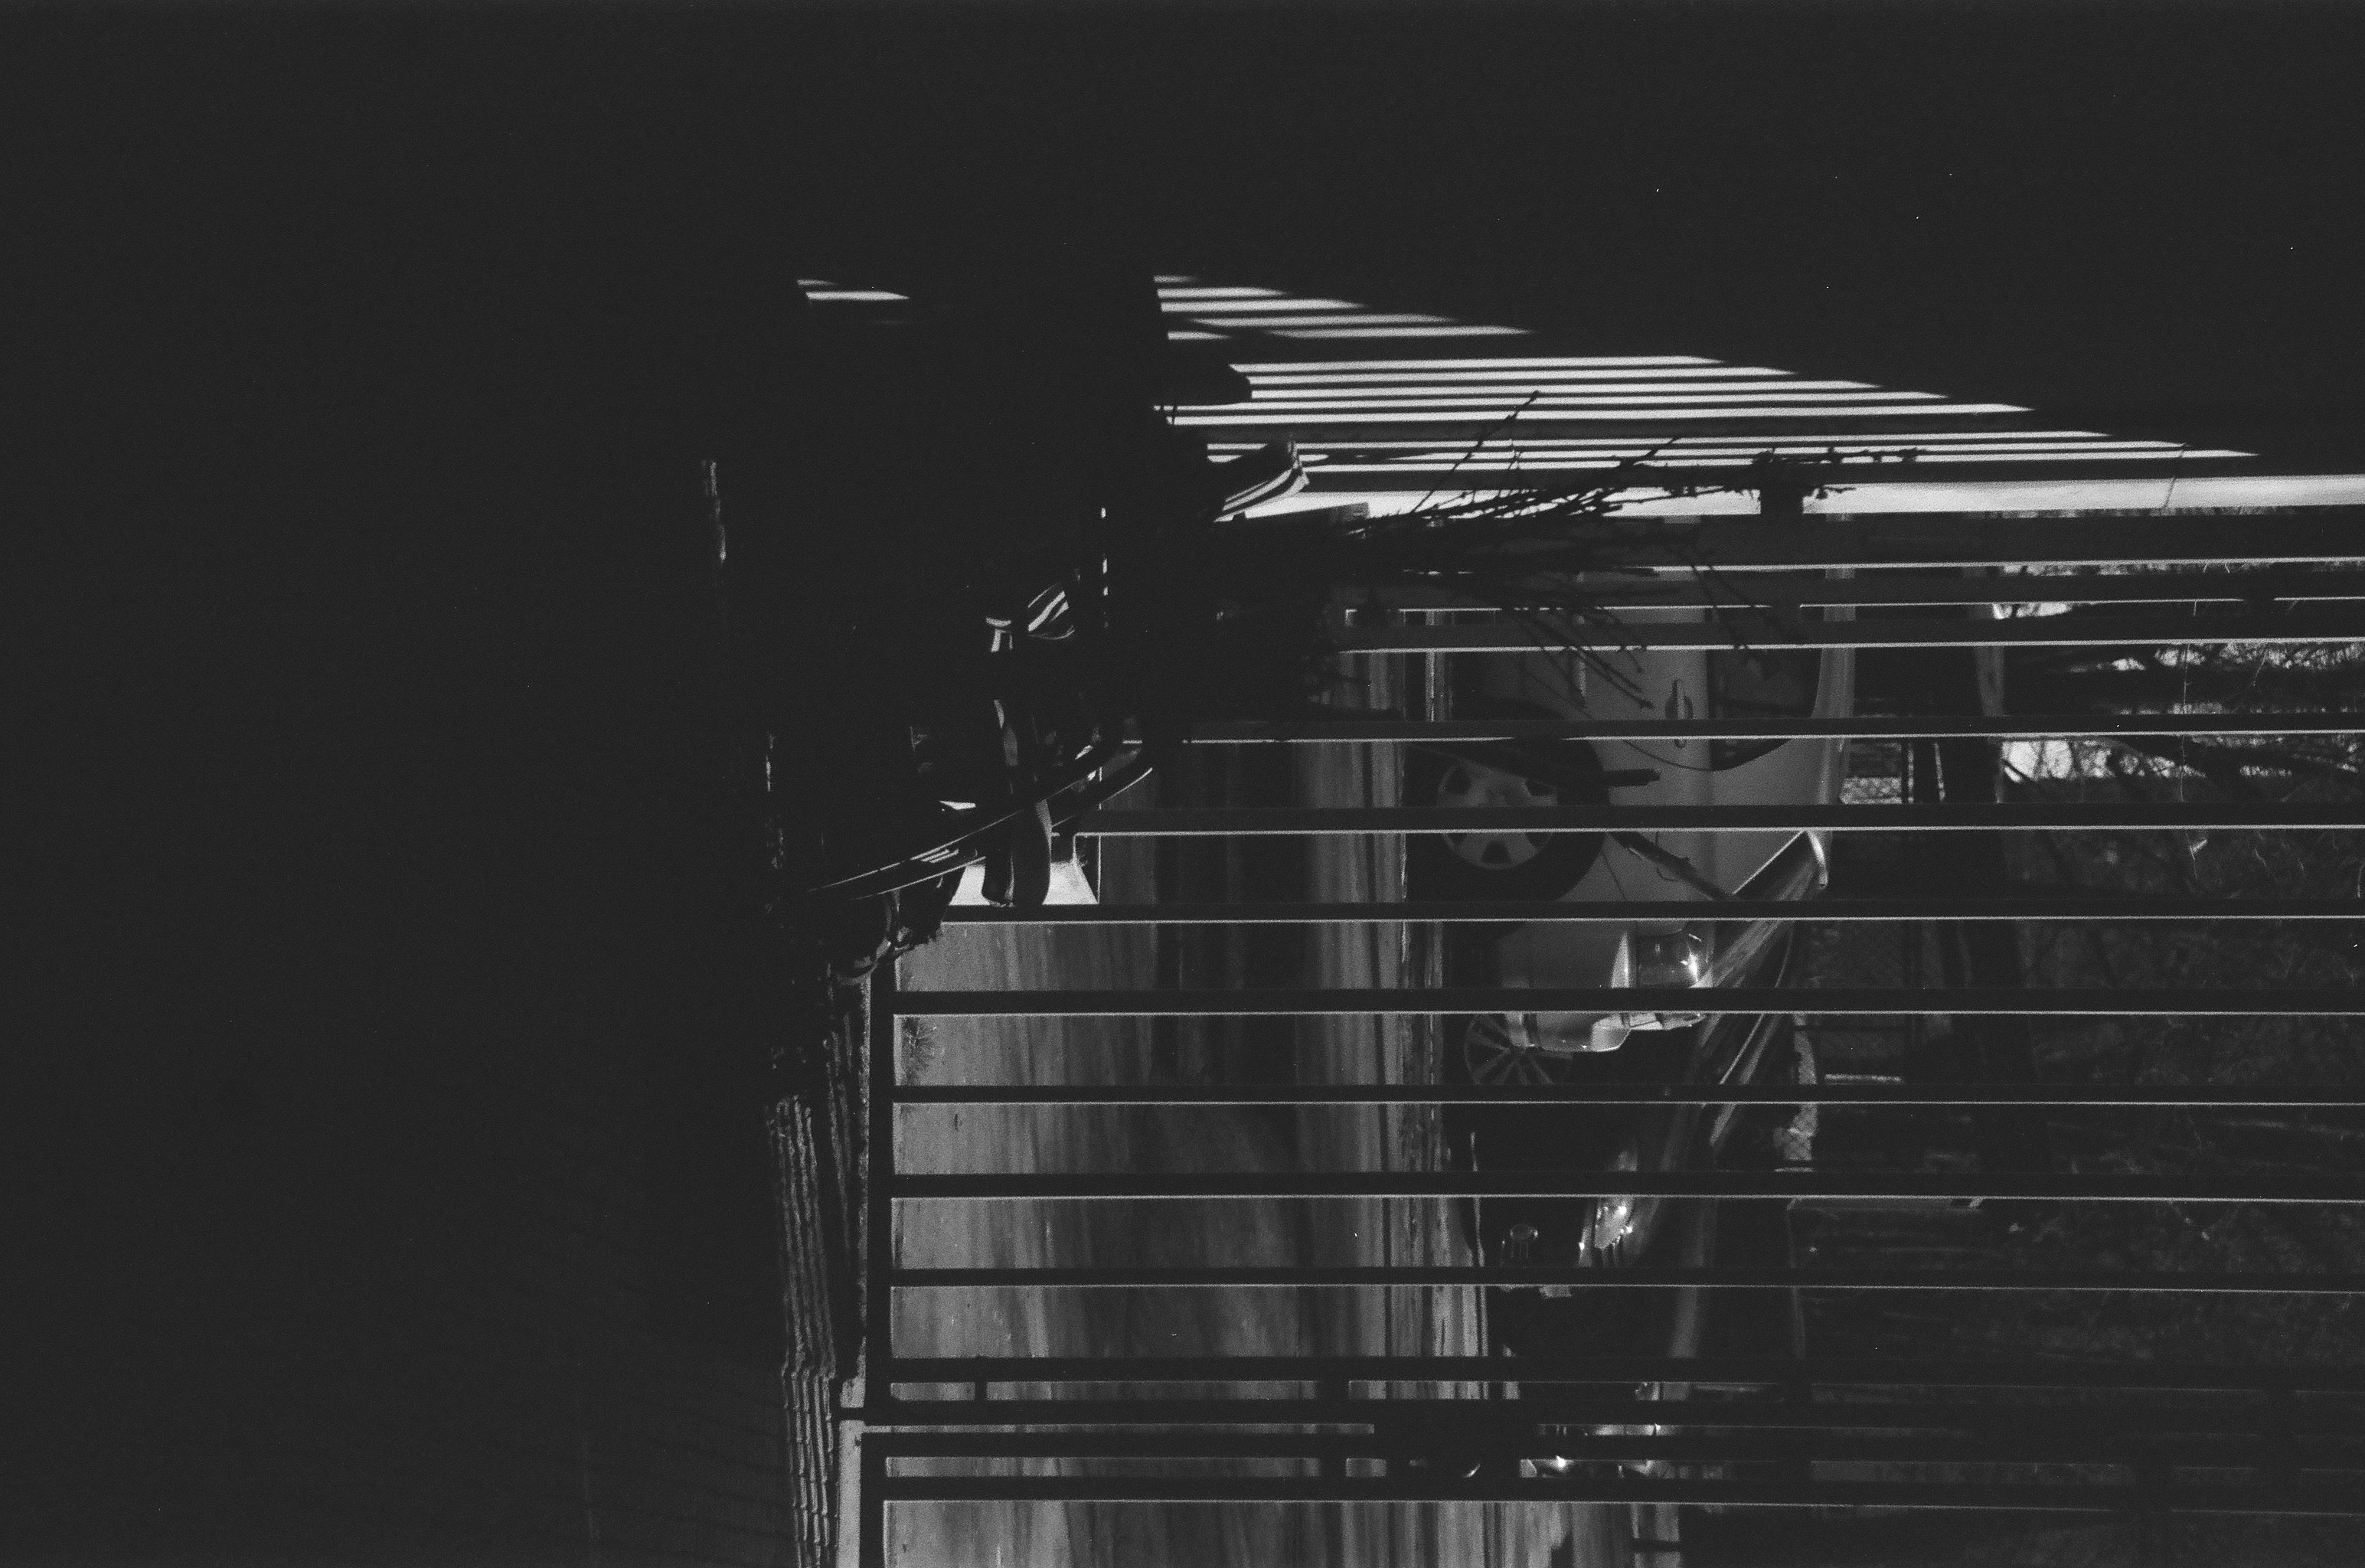
\includegraphics[angle=90, width=\linewidth, keepaspectratio]{Photos2/doswietlone_i_nie/analog6.jpg}
    \caption{Zdjęcie niedoświetlone.}
\end{figure}
\begin{figure}[H]
    \centering
    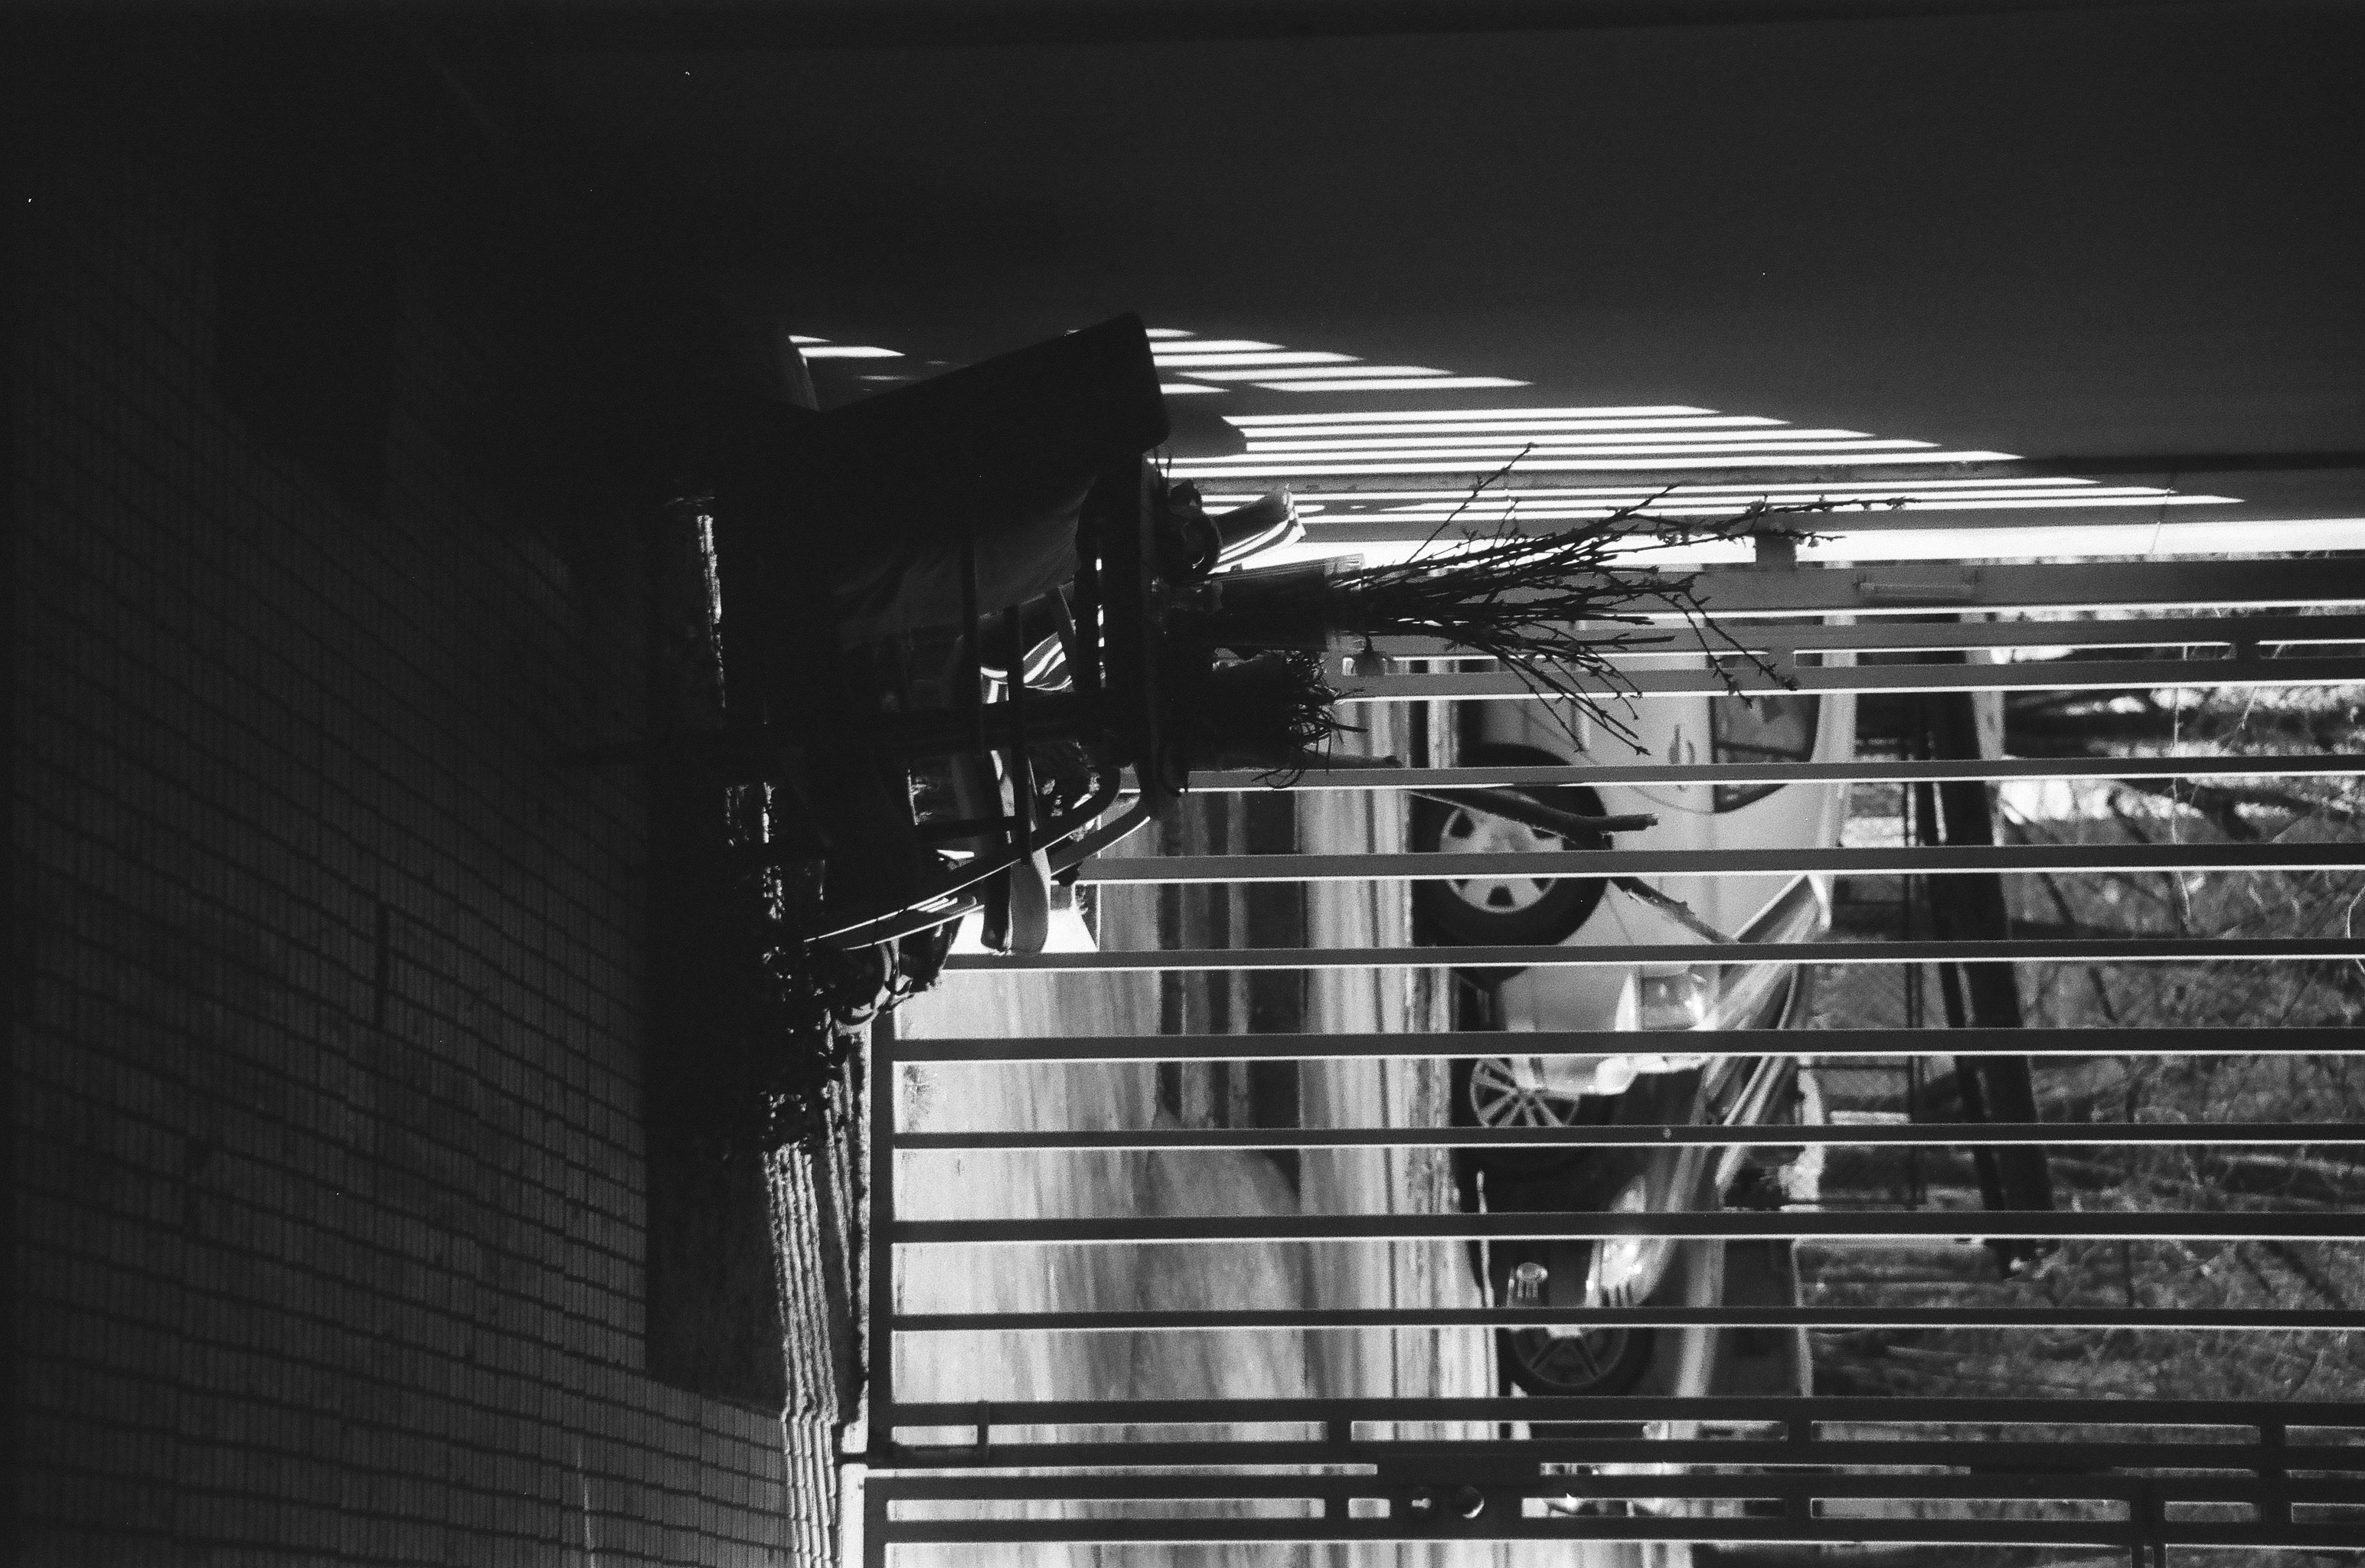
\includegraphics[angle=90, width=\linewidth, keepaspectratio]{Photos2/doswietlone_i_nie/analog7.jpg}
    \caption{...i to w punkt.}
\end{figure}

\newpage
\subsection{Zanieczyszczenia}
Prawie że cała nasza\footnote{nie jesteśmy wszak ani naukowcami, ani lekarzami.} codzienność
dzieje sie w niesterylnych warunkach. I jakkolwiek dla większości z nas nie jest to problem, są miejsca i sytuacje,
gdy prowadzi to do pewnych problemów. W powietrzu nas otaczającym jest pełno unoszących się zanieczyszczeń: włosów, kurzu, futra etc.

Problematyczne jest natomiast osadzanie się wspomnianej powyżej materii na zdjęciach i soczewkach -- która przenosi się na
skan tworząc nieestetyczne artefakty:

\begin{figure}[H]
    \centering
    \includegraphics[width=\linewidth, keepaspectratio]{Photos2/przed/gpt3.png}
    \caption{W skrajnych wypadkach może wyglądać to nawet tak.}
\end{figure}

\begin{figure}[H]
    \centering
    \includegraphics[width=\linewidth, keepaspectratio]{Photos2/przed/new1.jpeg}
    \caption{Choć bardziej częstym jest ten przypadek.}
\end{figure}

\begin{figure}[H]
    \centering
    \includegraphics[width=\linewidth, keepaspectratio]{Photos2/przed/new2.jpeg}
    \caption{A także taki.}
\end{figure}

\newpage
\section{Program i jego działanie}
Zbrojni w wiedzę co chcemy osiągnąć i zapas zebranych skanów zdjęć do testów wzięliśmy się do pracy
nad programem. Stworzyliśmy zaawansowany program, który w przypadku funkcjonalności
`anty--zanieczyszczeniowej' inteligentnie przeszukuje cały obszar zdjęcia, zaznacza artefakty,
a w następnej fazie działania usuwa je.

Przechodząc do szczegółów, działanie programu można opisać za pomocą kilku kolejnych faz działania\footnote{Algorytm
    przekształca zdjęcie z formatu RGB do formatu HSV (Hue, Saturation, Value) i działa tylko na Value, która definiuje jasność piksela w skali 0-255.} na przykładzie poniższego zdjęcia:

\begin{figure}[H]
    \centering
    \includegraphics[width=\linewidth, keepaspectratio]{Photos2/przed/gpt1.png}
    \caption{Przykładowe zdjęcie -- to za jego pomocą opiszemy działanie programu.}
\end{figure}

\subsection{Tworzenie maski}
\subsubsection{Rozmycie gaussowskie}
Pierwszym krokiem generowania maski jest stworzenie rozmycia gaussowskiego zdjęcia.

Wygładzanie gaussowskie jest efektem rozmywania obrazu za pomocą funkcji Gaussa,
która jest szeroko wykorzystywana w grafice komputerowej w celu uzyskania gładkiego
wygładzenia obrazu i wyciszenia szumu informacyjnego.

Za pomocą funkcji danej wzorem dla każdego piksela:
\begin{equation}
    G(x, y) = \frac{1}{2 \pi \sigma^2}e^{- \frac{x^2+y^2}{2\sigma^2}}
\end{equation}
gdzie $x$, $y$ to współrzędne danego piksel'a, a $\sigma$ oznacza odchylenie standardowe.\footnote{Źródło: \url{https://en.wikipedia.org/wiki/Gaussian_blur}}

\begin{figure}[H]
    \centering
    \includegraphics[width=\linewidth, keepaspectratio]{Photos2/gauss_blurr/gauss_blurr_gpt1.png}
    \caption{Zdjęcie po wykonaniu rozmycia gaussowskiego.}
\end{figure}

\subsubsection{Wykonanie różnicy}
Następnie odejmujemy od oryginału zdjęcia otrzymane w poprzednim etapie rozmycie.
Pozwala to na wykrycie najbardziej kontrastowych elementów zdjęcia.

\begin{figure}[H]
    \centering
    \includegraphics[width=\linewidth, keepaspectratio]{Photos2/difference/difference_gpt1.png}
    \caption{Zdjęcie po wykonaniu różnicy.}
\end{figure}

\subsubsection{Usunięcie ciemnych pikseli}
Zostawiamy tylko jasne piksele (według standardowych ustawień jest
to jasność powyżej 60) i nadajemy im maksymalną wartość 255.
Pozostałym pikselom ustawiamy jasność na 0.

\newpage
\subsubsection{Korekcja gamma}

Korekcja gamma jest techniką stosowaną w grafice komputerowej, której celem jest dostosowanie
jasności obrazu do ludzkiego nielinowego postrzegania światła. Korekcja gamma kompensuje ten
nieliniowy sposób widzenia, pozwalając na efektywniejsze wykorzystanie dostępnych poziomów jasności.

Korekcja gamma dokonuje transformacja jasności w następujący sposób:
\begin{equation}
    L'(x,y) = L(x,y)^{\gamma}
\end{equation}
gdzie:
\begin{itemize}
    \item $\gamma$ to współczynnik gamma,
    \item $L(x,y)$ to wartości jasności pikseli.
\end{itemize}

Wiedząc to, w tym etapie bierzemy ponownie oryginalne zdjęcie, wykonujemy
na nim korekcję gamma, a następnie na tym zdjęciu wykonujemy etapy 1-3.

Działanie to pozwala uwzględnić jak najwięcej artefaktów
-- znajdujących się także na jasnym tle.

\begin{figure}[H]
    \centering
    \includegraphics[width=\linewidth, keepaspectratio]{Photos2/gamma_corection/gamma_corection_gpt1.png}
    \caption{Po wykonaniu korekcji gamma i etapów 1-3.}
\end{figure}

\newpage
\subsection{Gotowa maska}
Po tym wszystkim otrzymujemy dwie podmaski (jedna robiona na oryginalnym
zdjęciu, a druga na jaśniejszym -- rozświetloną modulacją gamma).
Końcową maskę otrzymujemy biorąc wszystkie znalezione piksele z obu podmasek.

\begin{figure}[H]
    \centering
    \includegraphics[width=\linewidth, keepaspectratio]{Photos2/masks/final_mask_gpt1.png}
    \caption{Maska wykonana z oganianego zdjęcia}
\end{figure}
\begin{figure}[H]
    \centering
    \includegraphics[width=\linewidth, keepaspectratio]{Photos2/masks/second(gc)_mask_gpt1.png}
    \caption{Maska wykonana z zdjęcia rozświetlonego korekcją gamma}
\end{figure}


\newpage
\subsection{Działanie właściwe}
Mając wygenerowaną maskę właściwą, przechodzimy po wyznaczonych
przez nią pikselach na oryginalnym zdjęciu. Dla każdego piksela w
zaznaczonego w masce wyliczamy nową wartość jasności -- średnią z
jasności wszystkich (nie zaliczają się do tego pikseli wyznaczone
wcześniej przez maskę.) pikseli na odległości nie więcej 15 od aktualnie analizowanego.

Wynik finalny:
\begin{figure}[H]
    \centering
    \includegraphics[width=\linewidth, keepaspectratio]{Photos2/przed/gpt1.png}
    \includegraphics[width=\linewidth, keepaspectratio]{Photos2/po/gpt1.png}
    \caption{Przykładowe zdjęcie -- porównanie efektu przed i po.}

\end{figure}

\newpage
\section{Uwagi co do działania programu}
Przez to, że algorytm działa lokalnie (tylko w punktach wyznaczonych
przez maskę) nie wpływa on na ogólny wygląd zdjęcia.
Z tego też powodu możemy wykonywać program kilkukrotnie na zdjęciu
-- uzyskując lepsze efekty.

Końcowy algorytm składa się z pięciu iteracji opisanego wyżej algorytmu,
znacząco zwiększając szansę na usunięcie zanieczyszczeń.

Ponadto można uzyskać dodatkowe informacje o działaniu programu
i jakości zdjęcia -- za przykład funkcja: .countNoise()
zlicza ilość wyznaczonych przez maskę pikseli -- które są uznane za zanieczyszczenia.





\section{Dostępność programu}
Na chwilę obecną nasze rozwiązanie jest programem terminalowym,
działającym na systemie nie starszym niż Windows 10 -- choć istnieje
plan przeniesienia go także na inne popularne systemy operacyjne.

Tak samo pracujemy obecnie nad stworzeniem bardziej przystępnego interfejsu okienkowego.

Program dostępny jest na licencji \textit{open source} i jego kod źródłowy można znaleźć na GitHubie
pod adresem:
\begin{center}
    \url{https://github.com/ssk12o/PTI-Foto-Projekt}.
\end{center}




\newpage
\section{Wykorzystywane narzędzia}
W tej części naszego projektu korzystaliśmy z następujących narzędzi:
\begin{itemize}
    \item Programu i języka Matlab -- do analizy zdjęć;
    \item Języka C++ -- do napisania programu;
    \item Programu VS Code -- do tworzenia, edycji i dokumentacji kodu programu i raportów;
    \item Programu LibreOffice Calc -- do analizy części danych numerycznych;
    \item $\LaTeXe{}$ -- do przygotowania raportu;
    \item Strony Github i programu Git -- do udostępniania, dystrybucji i pracy nad kodem;
    \item 7zip -- do kompresji zdjęć;
    \item Google Drive -- do udostępniania plików;
    \item Skanera minilab Noritsu HS-1800 -- do wykonywania wysokiej jakości cyfrowych skanów zdjęć wykonanych techniką analogową;
    \item Aparatów:
          \begin{itemize}
              \item Canon EOS 300 z obiektywem Tamron 28-105mm 1:4-5.6 i kliszą Fomapan 400
              \item Fujifilm FinePix L55 Digital Camera -- Black (12MP, 3x Optical Zoom)
          \end{itemize}
\end{itemize}


\section{Podział obowiązków}
Na tym etapie projektu podzieliśmy się pracą, obowiązkami i zadaniami w następujący sposób:
\begin{itemize}
    \item Bartosz Wójcik -- wykonywanie, skanowanie i analiza zdjęć; opieka merytoryczna.
    \item Katarzyna Szwed -- tworzenie, analizowanie i pisanie algorytmu; korekta raportu.
    \item Natalia Szymańska -- pisanie raportu.
    \item Patrycja Szałajko -- zarządzanie pracą zespołu, kontakt z mediami.
    \item Aleksandra Wójcik -- skanowanie zdjęć rodzinnych w celu polepszenia ich jakości w końcowych etapach projektu.
    \item Karol Sęk -- tworzenie, analizowanie i pisanie algorytmu.
    \item Michał Juszkiewicz -- tworzenie, analizowanie i pisanie algorytmu.
    \item Filip Sajko -- pisanie raportu, implementacja w \LaTeX{}.
\end{itemize}


%                       Wersja alternatywna podziału obowiązków
% \section{Podział obowiązków}
% Na tym etapie projektu podzieliśmy się pracą, obowiązkami i zadaniami w następujący sposób:
% 
% \begin{table}[h!]
%     \centering
%     \renewcommand{\arraystretch}{1.3}
%     \begin{tabular}{|p{3cm}|p{7.5cm}|} \hline
%         \textbf{Imię i nazwisko} & \textbf{Zakres obowiązków}                                                               \\ \hline \hline
%         Bartosz Wójcik           & Wykonywanie, skanowanie i analiza zdjęć; opieka merytoryczna.                            \\ \hline
%         Katarzyna Szwed          & Tworzenie, analizowanie i pisanie algorytmu; korekta raportu.                            \\ \hline
%         Natalia Szymańska        & Pisanie raportu.                                                                         \\ \hline
%         Patrycja Szałajko        & Zarządzanie pracą zespołu, kontakt z mediami.                                            \\ \hline
%         Aleksandra Wójcik        & Skanowanie zdjęć rodzinnych w celu polepszenia ich jakości w końcowych etapach projektu. \\ \hline
%         Karol Sęk                & Tworzenie, analizowanie i pisanie algorytmu.                                             \\ \hline
%         Michał Juszkiewicz       & Tworzenie, analizowanie i pisanie algorytmu.                                             \\ \hline
%         Filip Sajko              & Pisanie raportu, implementacja w \LaTeX{}.                                               \\ \hline
%     \end{tabular}
%     \caption{Podział obowiązków w zespole projektowym.}
% \end{table}




\end{document}